\chapter{Motivation}
\label{chap:motivation}
In a world of ever growing data, we quickly come to a point where analytic computations on a single, local workstation are no longer feasible. To overcome the limited capabilities of a single machine, specialized frameworks, such as Apache Hadoop, have emerged and paved the way for big data analysis through distributed storage and computation across multiple computers.\\

One exemplary use case, where statisticians can benefit from a distributed setting, as provided by Hadoop, is the analyzation of stock exchange data. Market place organizers, such as Deutsche B\"orse, hold millions of historic transaction details for a great number of stocks. The size of such data sets can easily grow into the range of Petabytes, hampering local-only analyzation.
\\

The remainder of this paper is structured as follows: \Cref{chap:introduction} gives a general introduction of the programming language R and the Apache Hadoop framework, \Cref{chap:integration} describes how to utilize Hadoop from within R to combine their capabilities and \Cref{chap:example} covers a real world example from the field of stock trading in detail. \Cref{chap:conclusion} closes with a short conclusion.


\chapter{Background}
\label{chap:introduction}
After a brief introduction into the programming language R, this section gives an outline about the large-scale data management system Apache Hadoop and its underlying concepts for distributed data storage and data processing.

\section{R}
R~\cite{RLanguage} is a free programming language with a strong focus on statistical computing and graphics.
While a fresh installation of R provides only basic functionality, it's capabilities can easily be extended through extra packages~\cite{rPackages}. There is a strong community of R users actively involved in the development and maintenance of additional functionality to the R language. The distributed \ac{CRAN} platform currently (June 2016) lists more than 8500~\cite{CRAN} additional packages, while further packages can be found on repositories as \eg GitHub.

\subsection{RStudio}
While R comes with a command line interpreter, there exist powerful and productive user interfaces. Probably the most popular one is RStudio~\cite{RStudio}, which is open source and available for Windows, Mac and Linux. It comes in two editions: RStudio Desktop and RStudio Server, while the latter one runs on a remote Linux server and allows accessing RStudio using a web browser.

\section{Hadoop}
\begin{figure}[ht]
\centering

\includegraphics[width=0.50\linewidth]{content/images/Hadoop_logo}
\caption{Apache Hadoop~\cite{HADOOP}.}
\label{fig:hadoopLogo}
\end{figure}
Apache Hadoop is a large-scale data management system maintained and released by the Apache Software Foundation under open source licence. It is a framework designed for the distributed storage and processing of very large data sets (Petabytes) across computer clusters~\cite{HADOOP} and provides a highly extendable ecosystem as shown in \Cref{fig:ecosystem}. The projects official logo is shown in \Cref{fig:hadoopLogo}.

\begin{figure}[ht]
\centering
%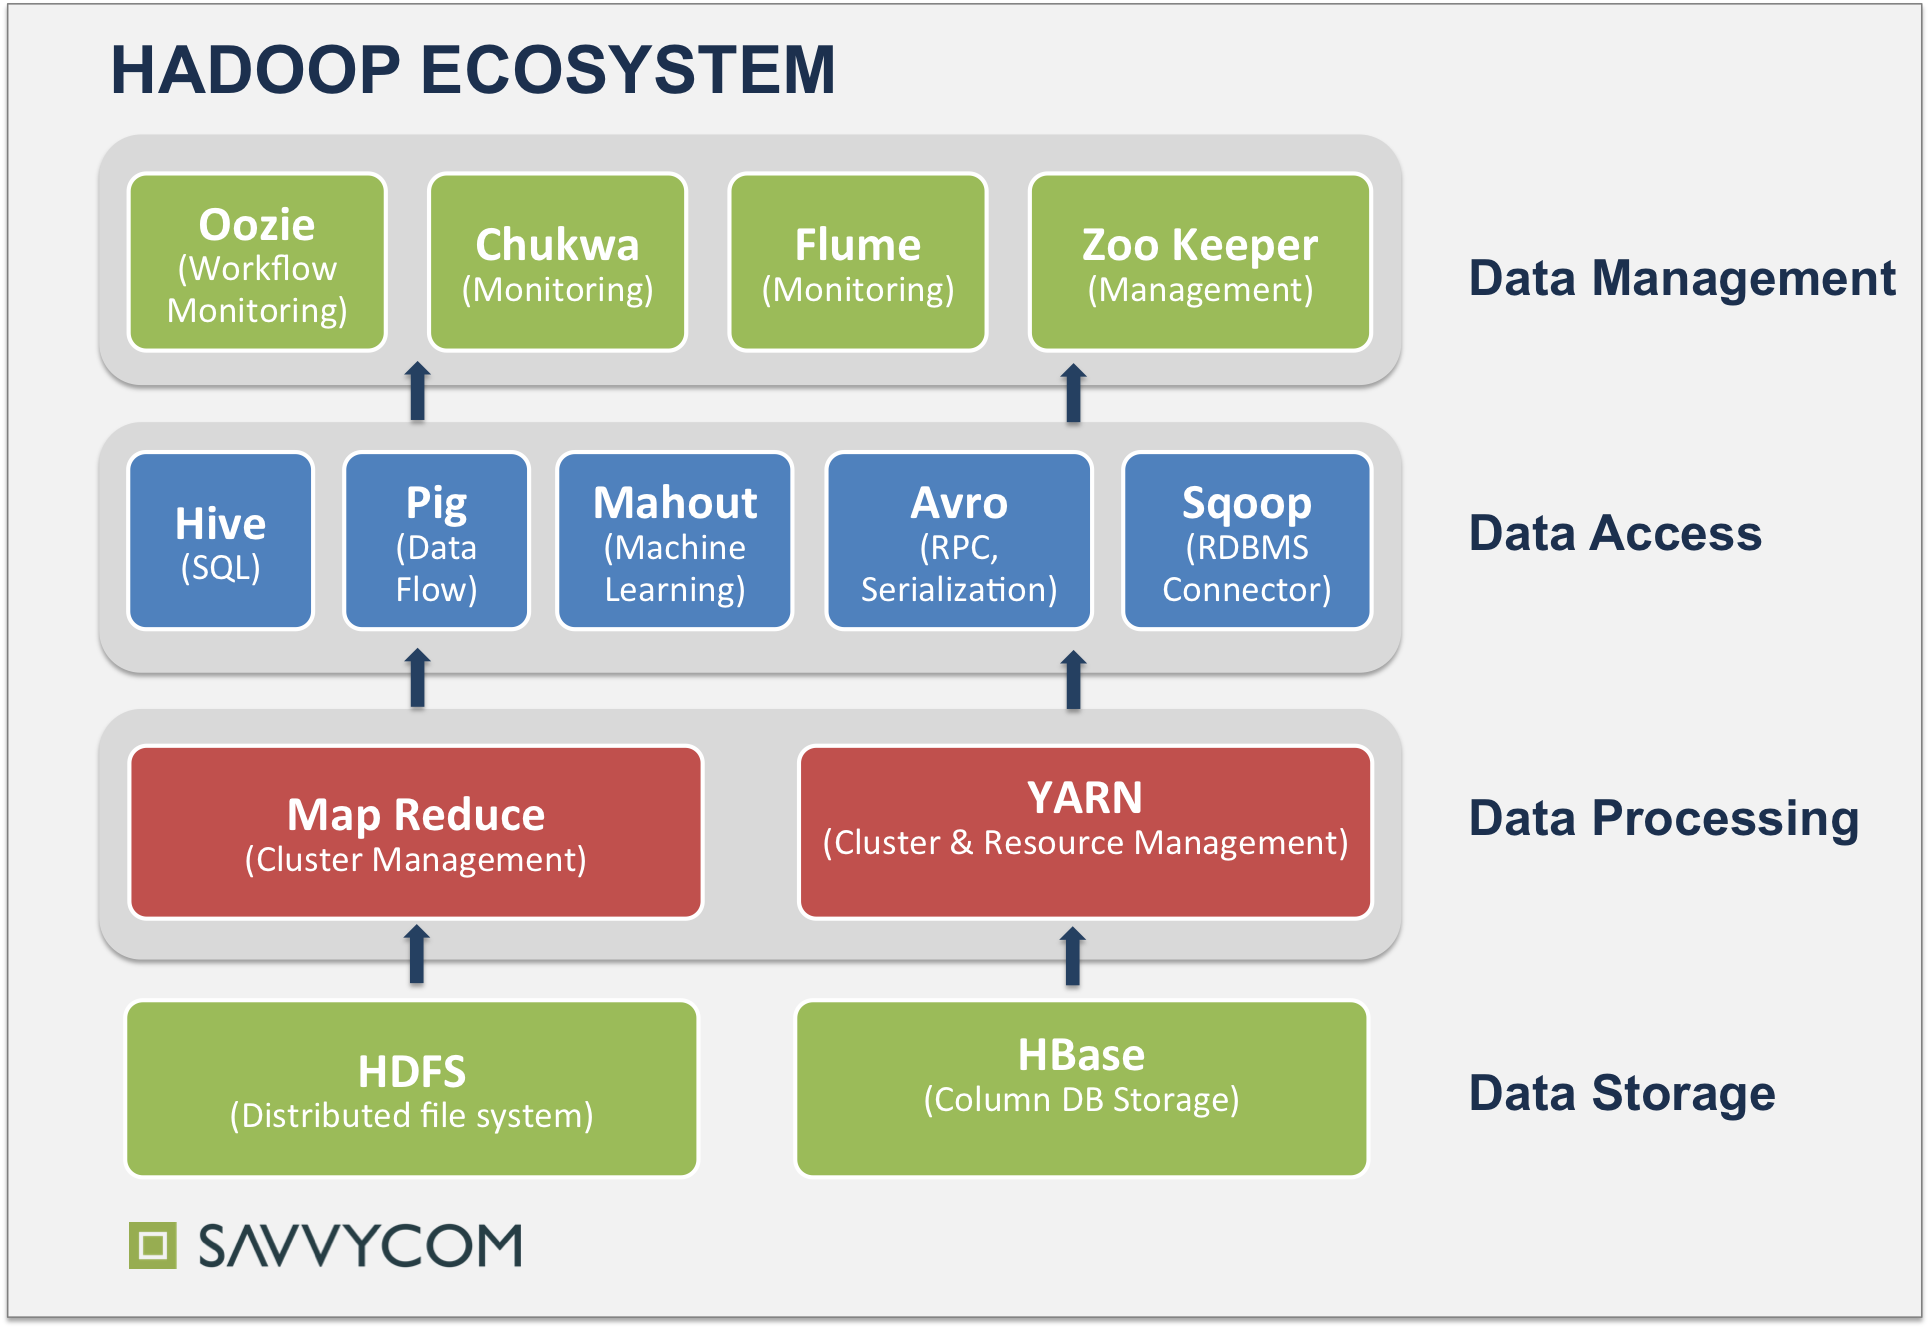
\includegraphics[width=0.60\linewidth]{content/images/HadoopEcosystem}\\
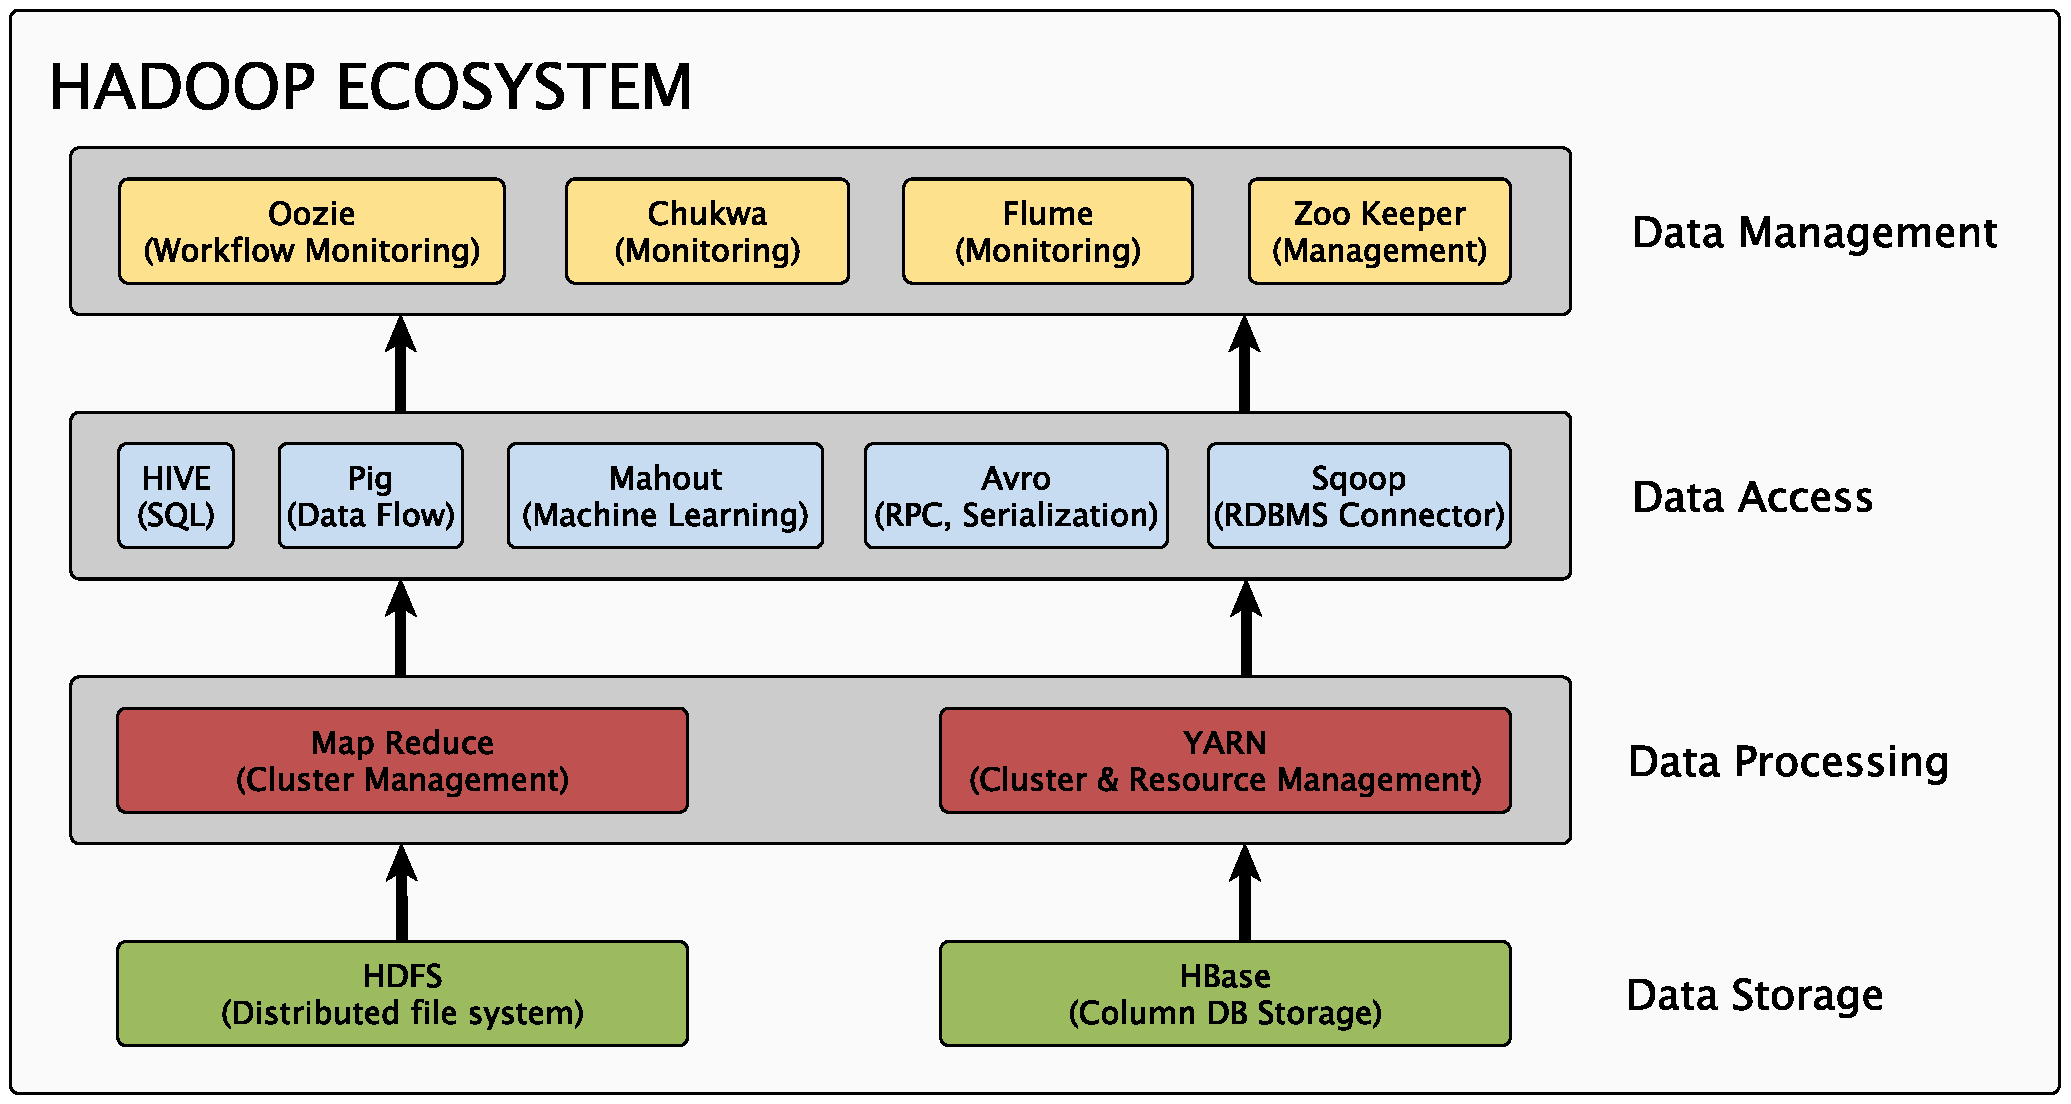
\includegraphics[width=0.70\linewidth]{content/drawings/hadoopEcosystem}

\caption{Hadoop Ecosystem.}
\label{fig:ecosystem}
\end{figure}

Built upon simple programming models, Hadoop can be scaled from single nodes to thousands of machines and runs on low-cost commodity hardware which is usually more vulnerable for failures than expensive, specialized hardware. To guarantee a highly-available service, the framework is designed to automatically detect and handle such failures.\\

What makes Hadoop different from traditional parallelism frameworks is its solution to the annoying I/O bottleneck typically arising in big data computations. Rather than bringing the data to the computing node, it brings the computation to the data. The fundaments of Apache Hadoop basically consists of the storage part \ac{HDFS} and the processing part MapReduce, which are in the focus of this paper.

\subsection{Hadoop Distributed File System (HDFS)}
The storage part, \ac{HDFS}, is a highly fault-tolerant filesystem designed to run on low-cost hardware which is inspired by the \ac{GFS}\cite{GFS}. \ac{HDFS} provides high-throughput access to application data and is tuned to support very large files. The files are split into large blocks (\eg 64~MB), replicated for reliability and distributed across various nodes in a cluster as illustrated in \Cref{fig:HDFS}.

\begin{figure}[ht]
\centering
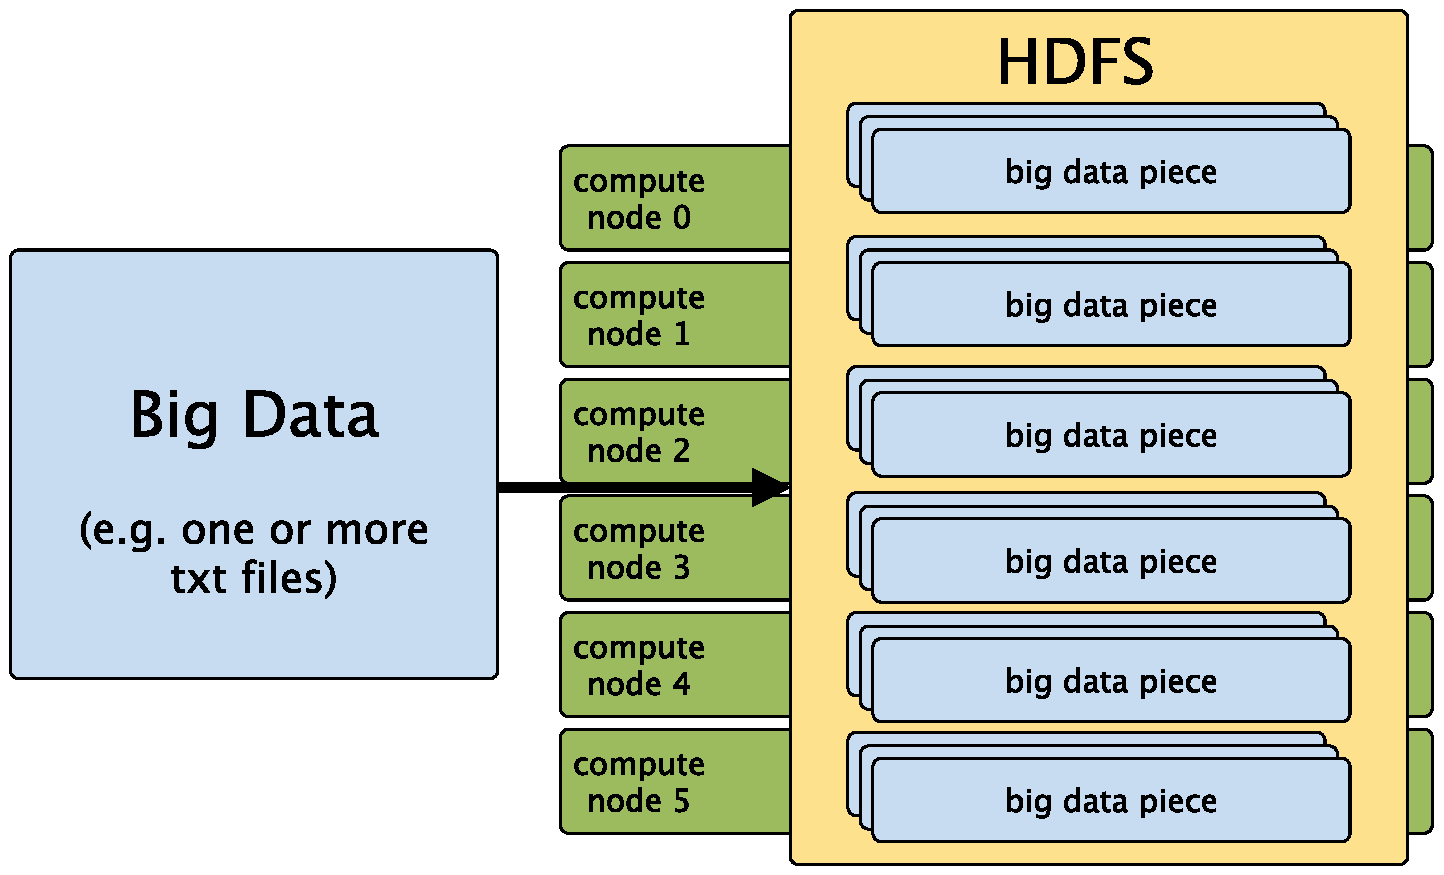
\includegraphics[width=0.50\linewidth]{content/drawings/BigDataDistribution}
\caption{File distribution across multiple physical compute nodes.}
\footnotesize 
\label{fig:HDFS}
\end{figure}
Typical file manipulation commands as e.g. \texttt{ls, mkdir, rm, mv, cp, cat, tail, chmod, ...} can be used to interact with files, while \ac{HDFS} takes care of recombining the data appropriately~\cite{lockwood}. These commands can be run via the Hadoop command  \texttt{hadoop dfs [GENERIC\_OPTIONS] [COMMAND\_OPTIONS]}.

\begin{tabular}[t]{ll}
Example & \texttt{hdfs dfs -ls /user/isresearch/}\\
 & \texttt{hdfs dfs -put ./1017\_01\_M\_08\_E\_20090331.csv /user/isresearch/}\\
\end{tabular}
\vspace{0.1cm}


\subsection{Hadoop MapReduce}
The processing part, Hadoop MapReduce, is an implementation of Googles MapReduce programming model~\cite{googleMapReduce} and is  composed of three phases:
\begin{description}
\item[Map()] In the first phase, each worker node applies the \emph{Map()} function to it's local part of the data. The data can be filtered and sorted in any desired form and will eventually be converted into zero or more key-value pairs.

\item[Shuffle()] In the second phase, the results from the previous \emph{Map()} phase are grouped according to their given key and stored back into the \ac{HDFS}. The Filesystem takes care of the redistribution of the intermediate results, such that all data of one key is located on the same physical node.

\item[Reduce()] In the last phase the worker nodes apply the \emph{Reduce()} function on each group of intermediate results individually and in parallel. The \emph{Reduce()} function performs a summary operation, such as counting the number of respective data points.
\end{description}

In contrast to traditional parallelism models, MapReduce performs the computation where the data resides, rather than transferring the data to the computation. As such, it avoids the previously mentioned I/O bottleneck, which arises from limited bandwidth and transportation cost induced by huge data files. Note that the individual phases must be complete before a succeeding phase can start. The typical MapReduce workflow is illustrated in \Cref{fig:mapreduceWorkflow}.

\begin{figure}[ht]
\centering
%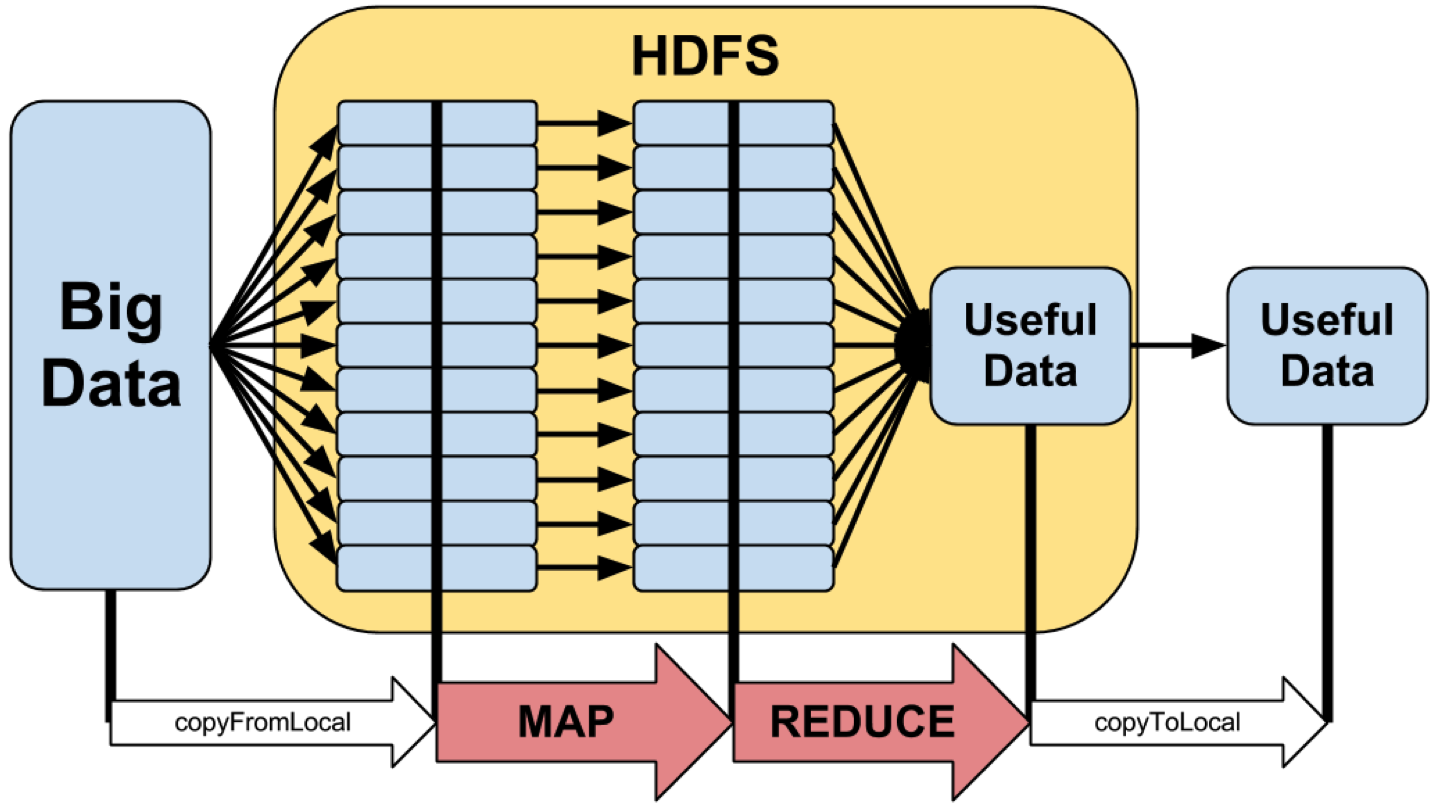
\includegraphics[width=0.60\linewidth]{content/images/mapreduce-workflow}\\
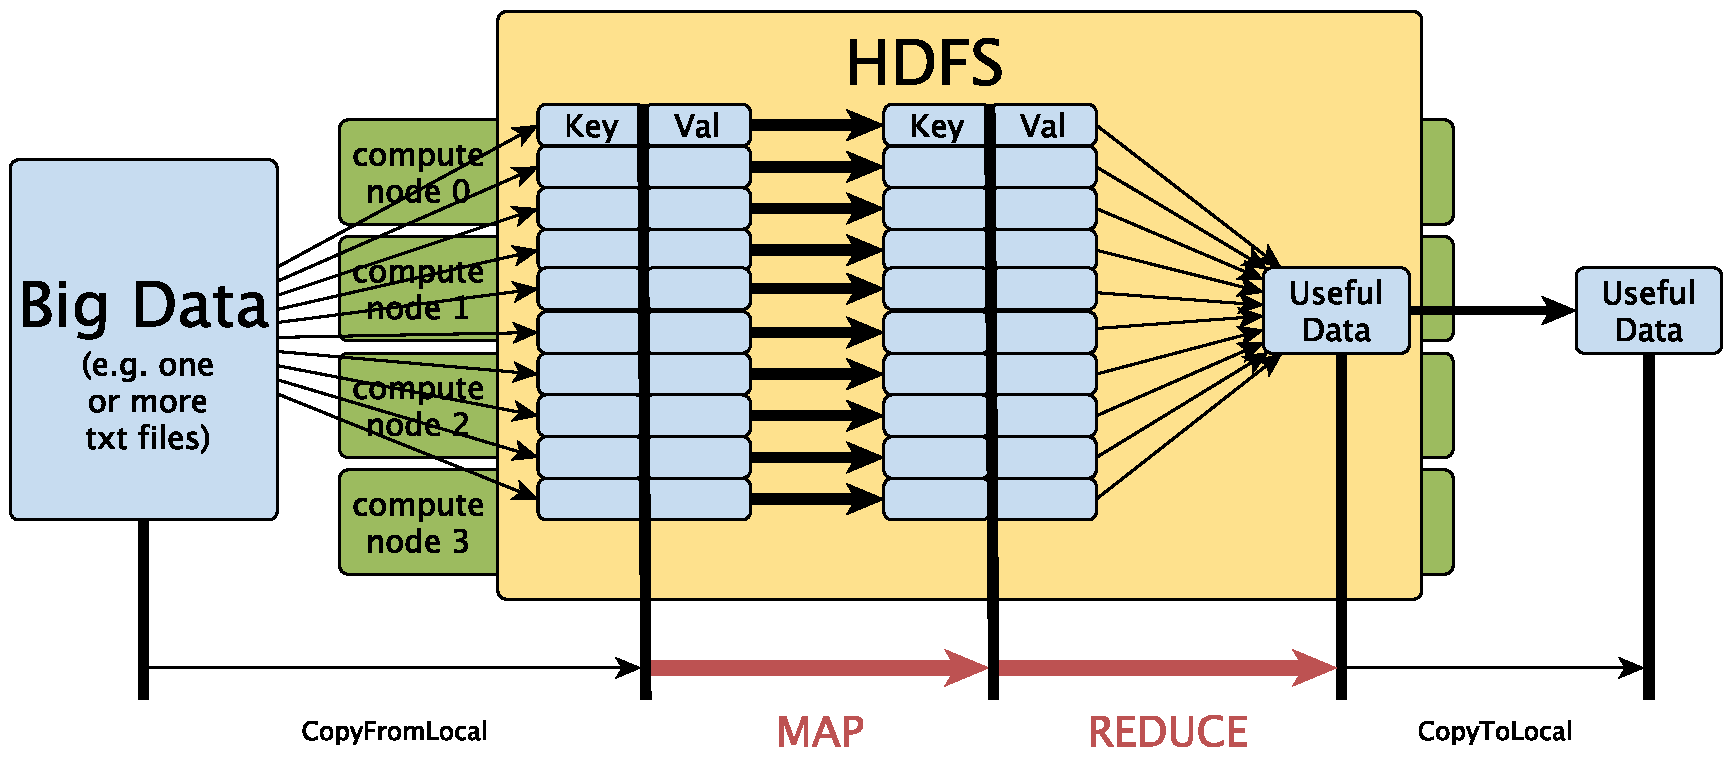
\includegraphics[width=0.70\linewidth]{content/drawings/MapReduceWorkflow}

\caption{MapReduce Workflow.}
\footnotesize 
\label{fig:mapreduceWorkflow}
\end{figure}


\subsubsection{Hadoop Streaming}
Hadoop Streaming~\cite{HadoopStreaming} is a generic API which comes with Hadoop. It allows Map and Reduce functions to be written in any language. Both functions read their respective input from stdin (line by line) and pass their output to stdout. The corresponding streaming format is shown in \Cref{lst:streaming}. The first part of each line until a delimiter (default: tab character) serves as the \emph{key}, while the rest of the line will be the \emph{value}. The output is always sorted by key.

\begin{lstlisting}[breaklines=true, caption=Default Hadoop Streaming format., escapechar=|, label={lst:streaming}]
key1 \t value1 \n
key2 \t value2 \n
key3 \t value3 \n
\end{lstlisting}
